\subsection{求解结果}

\renewcommand{\arraystretch}{1.25}
\setlength{\LTpre}{6pt}
\setlength{\LTpost}{6pt}

我们采用Python调用SciPy/HiGHS线性规划求解器，基于上述模型利用附件4的实时电价、附件2的负载与光伏实测数据以及附件3的光伏预报，重新求解问题二与问题三所对应的两类场景，年度计算从1月1日连续运行至年末，以1月形成历史信息与储电状态，费用统一统计2025年2月1日至12月31日共334天。为便于对照，以下将“在固定电价下按问题二策略求解”记为方案一、“在波动电价下按问题二策略求解”记为方案二、“在固定电价下按问题三策略求解”记为方案三、“在波动电价下按问题三策略求解”记为方案四。

\Needspace{0.35\textheight}
\begin{longtable}{>{\centering\arraybackslash}p{0.1579\textwidth}>{\centering\arraybackslash}p{0.1393\textwidth}>{\centering\arraybackslash}p{0.1207\textwidth}>{\centering\arraybackslash}p{0.1207\textwidth}>{\centering\arraybackslash}p{0.1207\textwidth}>{\centering\arraybackslash}p{0.1207\textwidth}}
  \caption{四个方案的全年购电费与风险指标对比}
  \label{tab:q4_cmp} \\
  \toprule
  方案 & 全年购电费(元) & 紧急购电量(kWh) & 紧急购电费(元) & 未消纳电量(kWh) & 费用增幅(\%) \\
  \midrule
  \endfirsthead
  \caption{四个方案的全年购电费与风险指标对比（续）} \\
  \toprule
  方案 & 全年购电费(元) & 紧急购电量(kWh) & 紧急购电费(元) & 未消纳电量(kWh) & 费用增幅(\%) \\
  \midrule
  \endhead
  \bottomrule
  \endfoot
  方案一（固定电价，问题二） & 13790848.69 & 75858.03 & 468467.64 & 2687529.82 & — \\
  方案二（波动电价，问题二） & 14526595.92 & 75033.76 & 491939.63 & 2623658.96 & +5.34 \\
  方案三（固定电价，问题三） & 13298484.49 & 42914.20 & 245780.57 & 2014393.07 & — \\
  方案四（波动电价，问题三） & 14018361.30 & 41588.56 & 246697.18 & 1965903.51 & +5.41 \\
\end{longtable}

我们由表\ref{tab:q4_cmp}可知，电价由固定机制切换为实时波动机制后，方案二较方案一增加735747.23元，增幅为\textbf{5.34\%}；方案四较方案三增加719876.81元，增幅为\textbf{5.41\%}。在相同电价环境下进一步比较两类完整策略，可评价滚动机制的综合费用表现。在购电费上升的同时，方案二的紧急购电量、未消纳电量分别较方案一减少824.27 kWh与63870.86 kWh，方案四的紧急购电量、未消纳电量分别较方案三减少1325.65 kWh与48489.56 kWh。

\Needspace{0.35\textheight}
\begin{longtable}{>{\centering\arraybackslash}p{0.1179\textwidth}>{\centering\arraybackslash}p{0.1451\textwidth}>{\centering\arraybackslash}p{0.1451\textwidth}>{\centering\arraybackslash}p{0.1270\textwidth}>{\centering\arraybackslash}p{0.1360\textwidth}>{\centering\arraybackslash}p{0.1088\textwidth}}
  \caption{波动电价下指定日期的购电与紧急购电结果}
  \label{tab:q4_day} \\
  \toprule
  日期 & 计划购电量 & 生效购电量 & 紧急购电量 & 方案 & 日购电费 \\
   & (kWh) & (kWh) & (kWh) & — & (元) \\
  \midrule
  \endfirsthead
  \caption{波动电价下指定日期的购电与紧急购电结果（续）} \\
  \toprule
  日期 & 计划购电量 & 生效购电量 & 紧急购电量 & 方案 & 日购电费 \\
   & (kWh) & (kWh) & (kWh) & — & (元) \\
  \midrule
  \endhead
  \bottomrule
  \endfoot
  2025-03-20 & 64505.11 & 64505.11 & 86.51 & 方案二 & 41921.38 \\
  2025-06-21 & 42284.43 & 42284.43 & 0.00 & 方案二 & 20377.80 \\
  2025-09-23 & 70341.18 & 70341.18 & 1.08 & 方案二 & 46368.53 \\
  2025-12-21 & 94463.38 & 94463.38 & 16.04 & 方案二 & 72005.59 \\
  2025-03-20 & 64098.58 & 62700.51 & 270.74 & 方案四 & 42686.63 \\
  2025-06-21 & 42171.14 & 42171.14 & 0.00 & 方案四 & 20175.42 \\
  2025-09-23 & 69677.93 & 69677.93 & 1.08 & 方案四 & 45618.55 \\
  2025-12-21 & 94107.16 & 94107.16 & 33.05 & 方案四 & 71402.26 \\
\end{longtable}

我们由表\ref{tab:q4_day}可知，四个指定日期的购电费差异较大：12月21日的日购电费为72005.59元与71402.26元，约为6月21日的3.5倍。方案四在6月21日、9月23日和12月21日分别比方案二节省202.38元、749.98元和603.33元，但3月20日多支出765.25元。3月20日生效合同较原计划下调1398.07 kWh，且发生270.74 kWh紧急购电；其余三个指定日未调整合同。

\begin{figure}[ht]
  \centering
  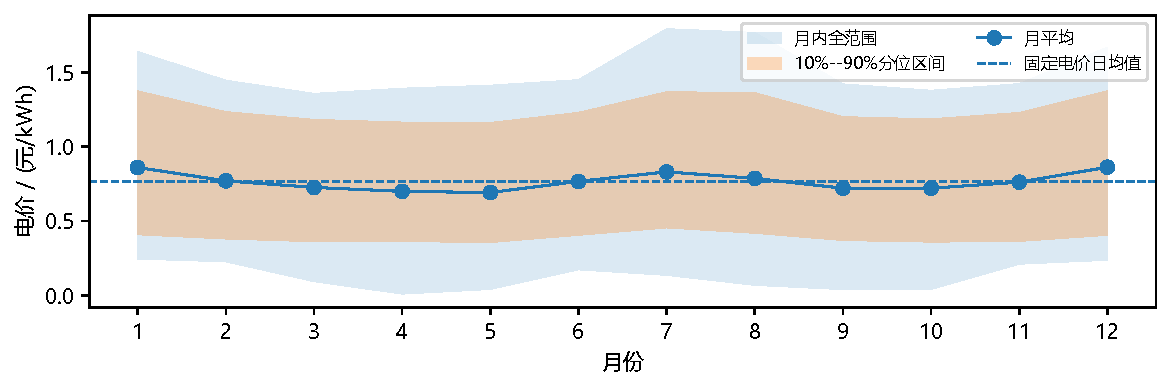
\includegraphics[width=0.86\textwidth]{figures/q4_price.pdf}
  \caption{全年电价的月度范围、分位区间与固定价日均值}
  \label{fig:q4_price}
\par\smallskip
\begin{minipage}{\textwidth}\small
图\ref{fig:q4_price}显示，实时电价的月度取值范围与分位区间存在明显差异，月内价格离散程度随月份变化。预测价格通过目标函数系数影响储能的充放电时序。
\end{minipage}
\end{figure}

% 指定日调度图与表格信息重复，正文保留价格波动、储能包络和风险图。

\begin{figure}[ht]
  \centering
  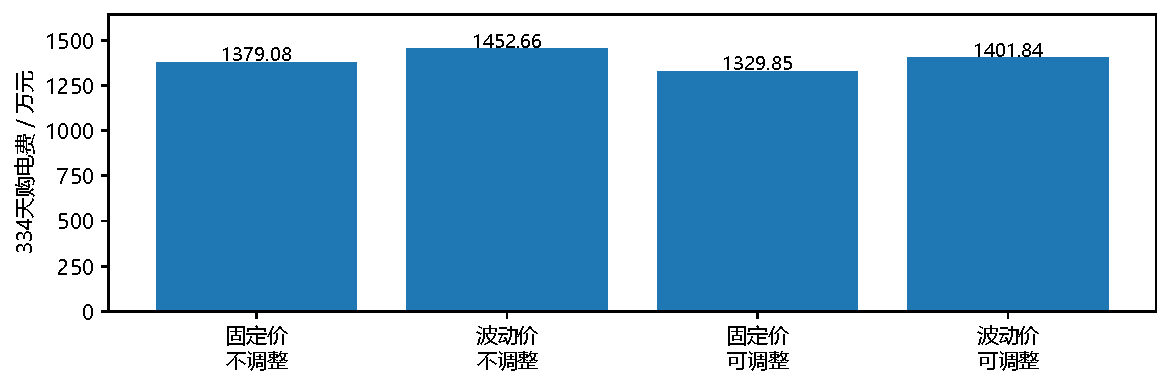
\includegraphics[width=0.86\textwidth]{figures/q4_cost.pdf}
  \caption{四个方案在334天评价区间的购电费对比}
  \label{fig:q4_cmp}
\par\smallskip
\begin{minipage}{\textwidth}\small
图\ref{fig:q4_cmp}显示，滚动调整方案的全年费用低于对应的日前方案，在固定电价和波动电价环境下分别节省\textbf{3.57\%}和\textbf{3.50\%}。
\end{minipage}
\end{figure}

\begin{figure}[ht]
  \centering
  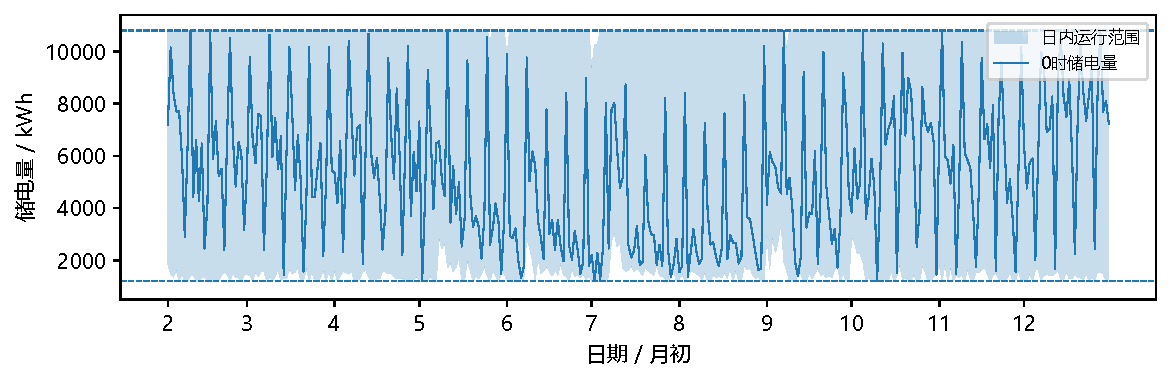
\includegraphics[width=0.84\textwidth]{figures/q4_soc.pdf}
  \caption{问题四跨日储能状态运行包络}
  \label{fig:q4_soc}
\par\smallskip
\begin{minipage}{\textwidth}\small
图\ref{fig:q4_soc}显示，储能状态始终处于1200至10800 kWh运行区间，各日储电量包络随供需和价格输入变化。
\end{minipage}
\end{figure}

\textbf{在波动电价下，正式可调整完整方案较不可调整完整方案节省508234.62元，节费3.50\%。}

\subsubsection{价格预测精度与跨月费用稳定性}
我们对问题四执行与问题三相同的逐日滚动起点回测。每日0时冻结未来24小时的价格预测，以附件4实现价格评价，得到MAE为0.04803元/kWh、RMSE为0.06570元/kWh、$R^2=0.9618$、WAPE为6.34\%。月度MAE介于0.03883与0.05917元/kWh之间。

为辨别偏差校正的作用，我们增加周同期季节性朴素预测作为基准，其MAE为0.04715元/kWh、RMSE为0.06535元/kWh。两种方法精度接近，周同期基准在本年度平均误差上略优。

我们将预测性能与运行性能分开统计，波动电价下完整滚动方案较对应日前方案的11个月费用均下降，月度降幅为1.19\%至8.51\%。这些月度差额反映完整策略在本年度实际价格与供需条件下的费用表现。
